\chapter{Описание реализации вспомогательного функционала}
\section{Получение требуемых разрешений от пользователя}
В соответствии с требованиями Google к безопасности пользовательских данных в рамках работы приложений в ОС Android для выполнения каких-либо действий или сбора каких-либо данных может потребоваться запросить на это разрешение у пользователя.

При этом, нельзя так просто взять и запросить разрешение. Перед этим его нужно объявить в файле AndroidManifest (см. Рис. \ref{fig:arch_uil_dol_dal}) который содержит некоторую метаинформацию о приложении, как-то:
\begin{enumerate}
	\item Название приложения.
	\item Список компонент (активности, сервисы, получатели сообщений, и т.д.).
	\item Название пакета с кодовой базой.
	\item Указание на первичную активность.
	\item Список разрешений, которые приложение будет запрашивать и задействовать.
\end{enumerate}
\dots и многое другое.
Так, в разрабатываемом приложении были указаны следующие разрешения:
\begin{enumerate}
	\item Для доступа к наиболее точной геолокации устройства:
	\begin{itemize}
		\item ACCESS\_FINE\_LOCATION
		\item ACCESS\_COARSE\_LOCATION
	\end{itemize}
	\item Для работы в фоне:
	\begin{itemize}
		\item ACCESS\_BACKGROUND\_LOCATION
		\item FOREGROUND\_SERVICE
	\end{itemize}
	\item Для определения физической активности пользователя устройства (на будущее):
	\begin{itemize}
		\item ACTIVITY\_RECOGNITION
	\end{itemize}
		\item Для уточнения геолокации и связи с сетевыми сервисами:
	\begin{itemize}
		\item ACCESS\_NETWORK\_STATE
		\item INTERNET
	\end{itemize}
\end{enumerate}

\begin{figure}[H]
	\centering
	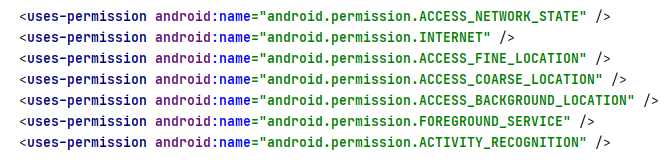
\includegraphics[width=\textwidth]{flesh/somefunc/manifest_permissions.png}
	\caption{\label{fig:manifest_permissions}Пример объявления разрешений в AndroidManifest.xml}
\end{figure}


После объявления разрешений требуется корректно их обработать в самом приложении – для каждого запрошенного разрешения проверить наличие разрешения от пользователя:
\begin{itemize}
	\item если разрешение есть \textendash\space продолжить выполнение инструкций приложения;
	\item если разрешения нет \textendash\space запросить его.
\end{itemize}


Проверку разрешений наиболее целесообразно производить в основной активности приложения. Однако, учитывая, что основная активность у нас сразу же инициализирует и отрисовывает фрагмент, отвечающий за отображение данных геолокации, было принято решение проверять разрешения в этом фрагменте.
Для проверки разрешения используется стандартный метод hasPermission контекста приложения (область методов и атрибутов приложения в конкретный момент времени, доступная в процессе выполнения приложения). 
В случае отсутствия разрешения инициализируется и отрисовывается один из фрагментов, содержащий макет с запросом на получение разрешения от пользователя. 

\section{Применение фрагментов}
Для замены фрагментов в содержимом, отображаемом на экране, используется встроенный объект supportFragmentManager~\autocite{android_fragment_manager}. Он позволяет в контексте атомарных транзакций управлять фрагментами. Алгоритм замены главного фрагмента фрагментом запроса разрешения выглядит следующим образом:
\begin{enumerate}
	\item Создать объект фрагмента, который следует отобразить на экране.
	\item Начать транзакцию.
	\item Передать инструкцию замены содержимого контейнера фрагмента созданным объектом.
	\item Сохранить операцию замены в конец стека операций транзакции.
	\item Применить транзакцию.
\end{enumerate}


\section{Организация хранения данных о геолокации устройства}
Как было описано в предыдущем разделе об архитектуре приложения, данные о геолокации хранятся в базе данных, доступ к которой производится через библиотеку Android Room, создающую некоторые абстракции для управления сущностями, объектами доступа к данным и объектами связи данных с макетом содержимого экрана.
Объект класса AppDatabase, наследующийся от системного RoomDatabase, реализует паттерн проектирования Singleton~\autocite{singleton}, доступен в единственном экземпляре на протяжении всей работы приложения и используется для следующих целей:
\begin{enumerate}
	\item Инициализация базы данных с нуля согласно автоматически сгенерированной схеме на основе известных приложению объектов типа Сущность.
	\item Инициализация репозитория с существующими данными, также реализующего паттерн проектирования Singleton, что делает его доступным в единственном экземпляре на протяжении всей работы приложения.
\end{enumerate}


\begin{figure}
	\centering
	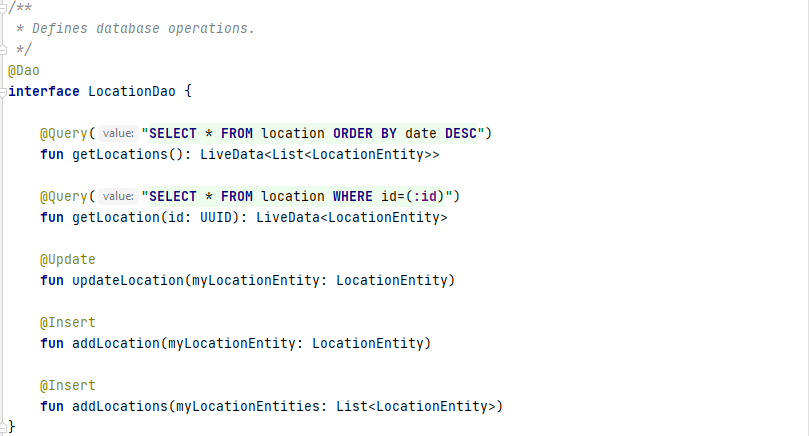
\includegraphics[width=\textwidth]{flesh/somefunc/location_dao.png}
	\caption{\label{fig:location_dao}Объявление методов объекта доступа к сохраненным данным геолокации}
\end{figure}

После инициализации базы и репозитория вся работа с данными производится с помощью методов объекта класса LocationDao (приведен на Рис. \ref{fig:location_dao}), который реализует CRUD модель доступа к содержимому репозитория.

\section{Получение данных о текущей геолокации устройства}
С помощью объекта LocationUpdatesBroadcastReceiver приложение подписывается на получение обновлений от сервиса геолокации Google Services – FusedLocationProviderClient.
Далее создается PendingIntent – ожидающее действие, которое при получении нового широковещательного сообщения с данными о геолокации запускает метод сохранения полученных данных в базу.
Доступ к сервису геолокации FusedLocationProviderClient производится через класс-обертку LocationManager, который отвечает за хранение флага активности отслеживания и настроек отслеживания, таких как частота отслеживания, приоритет получения данных и требуемая точность данных.

\section{Фоновое получение данных о геолокации}
В приложениях для ОС Android, как было описано ранее, используется концепция функциональных единиц – Activity (активностей). При этом в приложении всегда есть основная активность, которая запускается при открытии приложения. В ней инициализируют значения, запускают фоновые сервисы и указывают инструкции для отрисовки первичного содержимого экрана.
По умолчанию такая активность имеет название MainActivity. В ней мы создаем Intent («намерение» с некоторым действием), который запускает наш LocationService. 
При инициализации сервиса создается постоянное уведомление в шторку о работе приложения в фоне, в зависимости от версии ОС Android это делается по-разному.
Далее происходит запуск сервиса, в котором вызывается метод запуска отслеживания изменений геолокации из LocationRepository. Сервисы работают в фоне, поэтому им не требуется какое-либо представление в презентационном слое архитектуры приложения, при этом они могут обращаться к слою данных, что здесь и происходит.

\section{Связь данных с макетом содержимого экрана}
Именно за связь уже сохраненных данных о геолокации из базы и пользовательского интерфейса отвечает объект типа ViewModel – LocationUpdateViewModel: он содержит в себе вызовы соответствующих методов репозитория данных и больше ничего не делает.
Кроме того, для связи данных с макетом используются два механизма привязки объектов на этапе сборки:
\begin{description}
	\item[viewBinding] механизм привязки объектов макета к классу, содержащему инструкции по встраиванию макета в пользовательский интерфейс. Этот механизм позволяет не использовать устаревшую и неподдерживаемую конструкцию поиска объекта макета по его идентификатору – вместо этого после сборки проекта все элементы соответствующего макета доступны из автоматически генерируемого класса доступа к ним.
	\item[dataBinding] механизм действия, обратного viewBinding, позволяющий после сборки проекта использовать в макете содержимого пользовательского интерфейса содержимое объектов типа ViewModel.
\end{description}
Оба механизма включаются установкой соответствующих пакетов и заданием одноименных флагов в блоке buildFeatures конфигурационного файла системы сборки проекта Gradle – build.gradle (:app).


\section{Управление флагом активности отслеживания геолокации}
На основе LocationUpdateViewModel работает управление флагом состояния отслеживания: при нажатии на соответствующую кнопку в макете пользовательского интерфейса (включение/отключение отслеживания) производятся следующие действия:
\begin{enumerate}
	\item Запускается или останавливается сервис отслеживания.
	\item Вызываются методы LocationUpdateViewModel, запускающие или останавливающие отслеживание через отмену или активацию подписки на события изменения геолокации в LocationManager.
\end{enumerate}
